\documentclass[a4paper,11pt]{myreport}
%\documentclass{scrreprt}

\usepackage[dvipsnames]{xcolor}
\definecolor{souris}{gray}{0.19}
\definecolor{tagada}{RGB}{35,0,35}
\colorlet{bordeaux}{red!75!blue!25!darkgray}
\usepackage[hyperfootnotes=false]{hyperref}
\usepackage[toc,page]{appendix} 
\usepackage[utf8]{inputenc}
\usepackage[T1]{fontenc}
\usepackage{geometry}
\usepackage[export]{adjustbox}
\geometry{left=75pt,right=75pt,bottom=75pt}
\usepackage{a4wide}
\usepackage[francais]{babel}
\usepackage[babel=true]{csquotes} % csquotes va utiliser la langue définie dans babel
\usepackage{graphics}
\usepackage{movie15}
\usepackage{graphicx}
\usepackage{verbatim}
\usepackage{listings}
\lstdefinestyle{sharpc}{language=[Sharp]C, frame=lr, rulecolor=\color{blue!80!black}}
\usepackage[capbesideposition=bottom]{floatrow}
%\floatsetup{capposition=bottom}
\usepackage{caption}
\usepackage{color}
\usepackage{fancyhdr}
\usepackage[bottom]{footmisc}


\pagestyle{fancy}
\renewcommand{\footrulewidth}{1pt}
\fancyfoot[C]{\textbf{page \thepage}} 
\fancyfoot[L]{Projet 2A Informatique}
\fancyfoot[R]{Emmanuel Breton\--\--Belz}
\renewcommand{\footrulewidth}{0.7pt}
%\usepackage{syntonly}
%\newenvironment{DocStage}
%\syntaxonly
%%\setlength{\oddsidemargin}{dim souhaitée}
%%\setlength{\evensidemargin}{dim souhaitée}
%%\setlength{\textwidth}{dim souhaitée}
%%\setlength{\headheight}{dim souhaitée}
%%\setlength{\topmargin}}{dim souhaitée}
%%\setlength{\footskip}{90pt}

\setcounter{tocdepth}{2}
 \hypersetup{	
colorlinks=true, %colorise les liens 
breaklinks=true, %permet le retour à la ligne dans les liens trop longs 
urlcolor= blue, %couleur des hyperliens 
linkcolor= tagada ,	%couleur des liens internes 
citecolor=back,	%couleur des références 
pdftitle={Rapport de projet 2A}, %informations apparaissant dans 
pdfauthor={Emmanuel Breton\--\--Belz}, %les informations du document 
pdfsubject={Projet 2A}	%sous Acrobat. 
} 
\title{Jeu vidéo pédagogique utilisant la technologie Oculus VR}
\author{Emmanuel Breton\--\--Belz}


\begin{document} % ------------------------begin---------------------------------------
\def\siecle#1{\textsc{\romannumeral #1}\textsuperscript{e}~si\`ecle}

%reglages pour l’insertion de code
\lstset{language=Java,
basicstyle=\normalsize, % ou ça==> basicstyle=\scriptsize,upquote=true,
aboveskip={1.5\baselineskip},
columns=fullflexible,
showstringspaces=false,
extendedchars=true,
breaklines=true,
showtabs=false,
showspaces=false,
showstringspaces=false,
identifierstyle=\ttfamily,
keywordstyle=\color[rgb]{0,0,1},
commentstyle=\color[rgb]{0.133,0.545,0.133},
stringstyle=\color[rgb]{0.627,0.126,0.941},
}
\nopagebreak[3]


%\maketitle -------------------------------- premiere page
%%\setlength{\textheight}{28cm}
%%\setlength{\topmargin}{-5pt}

\makeatletter

  \begin{titlepage}
  \centering
      {\large \textsc{école nationale supérieur d'ingénieurs de caen}}\\
      \textsc{Dans le cadre du projet 2A}\\
    \vspace{1cm}
    \vspace{1cm}
      {\large\textbf{	\@date\\
      \LARGE{Rapport projet de 2\up{ème} année}}}
      
    \vfill
      
\includegraphics[width=0.25\textheight,center]{./images/LogoEnsicaenSansTexte.jpg}
    \vfill
       {\LARGE \textbf{\@title}} \\
    \vspace{1em}
        {\large \@author} \\
    \vfill

        
\includegraphics[width=0.25\textheight,left]{./images/oculus_logo.jpg}
        
\includegraphics[width=0.25\textheight,right]{./images/Unity_3D_logo.png}

  \end{titlepage}
\makeatother
%\end --------------------------------------------------------------------

%table des matières :
\setlength{\textheight}{26cm}
\setlength{\topmargin}{-2cm}

\tableofcontents


\newpage
\section*{Remerciements}
\par Tout d'abord nous tenons à remercier M. Lebrun pour nous avoir proposer le projet. Pour son suivi, la documentation et les conseils qu'il nous a fourni.
Pour nous avoir prêter l'oculuse VR pendant plusieurs semaines pour faire des tests.


\chapter{Introduction}
\par Le projet Oculus VR consiste en la réalisation d'un jeu à but pédagogique. Destiné à la promotion de l'école lors des journées portes ouvertes et des journées de l'étudiant en fin d'année 2015.
\par La réalisation du projet comprend l'utilisation de la technologie de réalité augmenté \''Oculus VR V2\'' détenu aujourd'hui par le groupe Facebook. Le modèle d'essaye appartient au laboratoire de recherche de l'ENSICAEN. Prêté pour le projet par Gilles Lebrun lors de nos tests.
\begin{figure}[h] 
	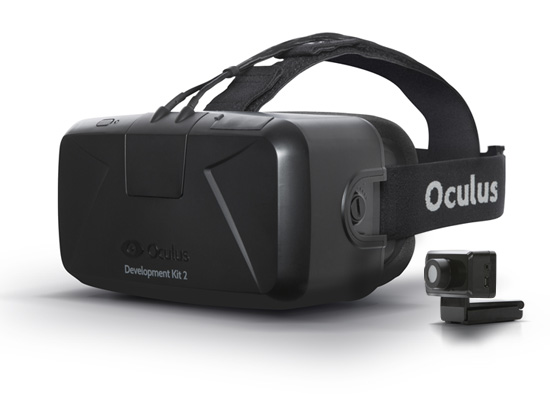
\includegraphics[scale=0.70]{./images/dk2-product.jpg}
	\caption{Casque Oculus VR kit de developpement version 2}
\end{figure}


\chapter{Contexte}
\par Aujourd'hui les jeux vidéos étant un média incontournable, beaucoup de société s'oriente vers l'utilisation de ceux-ci pour promouvoir, divertir, instruire le grand public. Notre projet ce situe entre le ludisme et la pédagogie et évidement, doit promouvoir en un sens, les compétences acquises lors de la formation à l'école.
\par Pour ce faire nous avons accès à une technologie remise au goût du jour il y a 3 ans, grâce à une campagne Kickstarter\footnote{Kickstarter : Plateform collaborative de participation en ligne à des projets divers.} : La réalité augmentée.

\section*{Jeu}
\par Notre jeu consiste à réaliser un algorithme à l'aide de cubes de différents couleurs. Évidemment il ne s'agit pas de les placer dans n'importe quel ordre pour que cela fonctionne.\\
On a donc pour référence, des cubes de couleur dans une zone dédiée, qui nous indiquent quel résultat on doit obtenir. On aussi des emplacement labellisés qui permettent de se faire une idée du type de cube à déposer pour que cela fonctionne. 
\begin{figure}[h]
	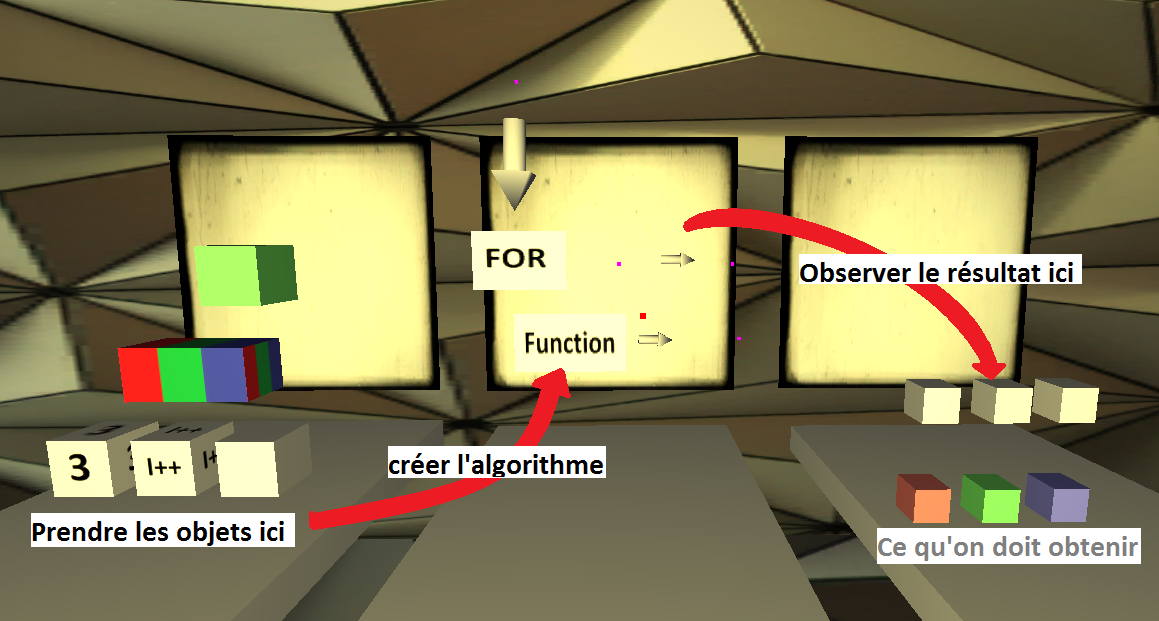
\includegraphics[scale=0.50]{./images/jeu.png}
	\caption{Schéma expliquant le principe du jeu}
	\end{figure}

\chapter{Réalisation}
\section{Outils}
\subsection{Choix du moteur}
\par Le choix du moteur\footnote{moteur de jeu : Logiciel permettant de réaliser des jeux vidéos grâce à une base logiciel conséquente, le code qu'on y ajoute et éventuellement une interface graphique et des scripts pré-existants.} est une partie important du projet. Même si avant même de commencer le projet nous avions déjà une idée du moteur que nous souhaitions utiliser, nous avons joué le jeu et essayer les deux logiciels. \`A savoir Blender Game Engine, un logiciel gratuit qui utilise python pour le rendu et Unity qui est un peu plus reconnu dans le monde professionnel mais payant. Unity prend en charge le JavaScript, le Boo et le C\# comme langage de programmation.

\par Comme nous sommes plus à l'aise avec le Java Unity marque un point avec le C\#, qui est facile à prendre en main quand on connait le Java. Ensuite lors de nos tests nous avons remarqué que l'interface de Blender est difficile à prendre en main. Elle nécessite de prendre en main un minimum de raccourcis clavier. Sans quoi les dizaines de boutons de l'interface sont un problème. Nous n'avons donc jamais produire un jeu en python avec Blender en une semaine de tests.
\par Par contre Unity est très facile à prendre en main. L'interface est assez agréable et simple d'utilisation.
\\Au final, voici la liste des avantages et inconvénients de chacun des deux logiciels :

  \begin{description}
  	\item \textbf{Blender Game Engine :}
  	\begin{itemize}
  		\item Interface difficile à prendre en main.
  		\item Reprendre le python pour programmer.
  		\item Pas d'intégration \''simple\'' de l'oculus.
  		\item Pas d'éditeur de script convivial.
  		\item Gratuit.
  		\item Beaucoup de tutoriels et d'aide sur internet.
  		\item Un mode pour la modélisation et un mode pour créer des jeux.
  	\end{itemize}
  	\item \textbf{Unity 3D :}
  		\begin{itemize}
  			\item Pas de mode dédié à la modélisation d'objets.
  			\item Payant.
  			\item MonoDevelop\footnote{MonoDevelop : IDE proposé par unity pour éditer les scripts qu'on attache au jeu.} peu pratique.
  			\item Kit d'intégration oculus développé pour Unity 3D.
  			\item Facile à prendre en main.
  			\item Possibilité de développer avec un langage objet (C\#).
  			\item Compatible avec Visual Studio.
  		\end{itemize}
  \end{description}
  
  \par Après s'être renseigner nous avons vu qu'il était possible de travailler à sur Unity sans payer (version d'évaluation). Comme le projet n'est pas utilisé à des fins commerciales, pas de soucis.
  \par Nous avons donc choisi Unity couplé au C\# pour les scripts. Nous détaillerons ce point juste après.
  
  \subsection{Le langage de programmation}
  \par Le langage de programmation ne nous été pas imposé. Donc nous nous sommes tournés rapidement vers le plus familier, le C\#. Un langage objet qui ressemble beaucoup au Java. Utilisé beaucoup pour développer des application pour Windows.
  \par Nous avons aussi testé le JavaScript mais pas le Boo. En récupérant des morceaux de codes sur internet (souvent disponible dans les 3 langages) on peut facilement porter un script d'un langage à un autre.
  Par contre on ne peut pas faire appel à un script JavaScript dans un script C\# par exemple. Donc il faut que le langage de programmation soit unifié.


\subsection{Environnement de développement}
\par Comme nous l'avons précisé plus tôt, Unity propose un environnement de développement (MonoDevelop). Il est sommaire mais plutôt efficace. Cependant il n'est pas parfaitement au point et laisse à désirer parfois.
Comme nous développons sous Windows, VisualStudio Community (pour la version gratuite) est disponible. Et il propose un pluging pour Unity ce qui fut une fort bonne nouvelle.
\par Ce pluging donne accès à des fonctionnalités comme l'attachement du script à Unity pour détecter les erreurs liés à la bibliothèque de Unity sans lancer le jeu. Une autocomplétion qui prend aussi bien en charge le C\# que la bibliothèque Unity, ce qui n'est pas le cas de MonoDevelop. Et un gestionnaire de version plus poussé que sur MonoDevelop mais qui laisse assez septique parfois tout de même.
Au final, pour la gestion de version, GitShell et les linges de commande étaient nettement plus efficace. Le dépôt GitHub est disponible \href{https://github.com/manumanmax/SeriousVR.git}{ici}.

\section{Développement}
\subsection{Prise en main}

\par Nous avons commencé par une longue phase de prise en main. D'abord de l'interface de Unity, ce qui fut assez rapide. Puis des scripts, ce qui prit beaucoup plus de temps.
Unity propose tout d'abord une classe MonoBehavior. Celle-ci implémente les méthodes classiques comme \''start\'' et \''update\'' qui sont respectivement lancées à l'instanciation de la classe et toute les frames\footnote{Frame: Anglissisme qui désigne une image générée par le jeu. Qui s'affiche entre 30 et 60 fois par seconde généralement.}. 
L'oculus VR nous a aussi pris beaucoup de temps. C'est une technologie assez capricieuse car il faut faire attention à la compatibilité des pilotes. Que l'application dédiée soit installée sur un système d'exploitation sans trop de virus. Il ne faut pas de résolution d'affichage ou propriété d'affichage un peu exotiques. Sinon même un simple jeu de démonstration ne pourra pas se lancer correctement.
Et même une fois avec testé une application on ne peut pas être certain que cela dur.
\par Lors de nos tests nous avons quand même pu lancer la démonstration \''Toscany\'' offerte dans l'API Oculus. Nous avons pu remarquer que le système requière un ordinateur avec une carte graphique assez puissante (Gefore GTX récent ou équivalent, parfaitement suffisant). Et on se laisse prendre au jeu de la perspective facilement. Attention tout de même à ne pas en abuser car des effets de nausées peuvent être ressentis rapidement. 
Quand bien même, une fois la caméra intégrée à une scène Unity et l'exportation faite. Nous avons pu voir qu'il était simple d'utiliser l'Oculus avec Unity 3D.
\subsection{Sprints}
\par Nous avons tenté de faire un développement régulier mais ce ne fut pas évident avec les cours en parallèle du projet. Le développement c'est plus fait sous forme de sprints.
D'abord pour nos différents tests, puis pour la conception des différentes briques du jeu final.
Chaque sprint était dédié à une fonctionnalité et ne durait pas plus de quelques heures. Ce qui, au final, répartissait bien la charge de travail, permettait d'implémenter des composants atomique et de mieux apprécier  l'avancement du projet.

\subsection{Répartition des tâches}
\par Nous nous sommes réparti les test, Benjamin plutôt le côté modélisation et affichage de labels, Emmanuel plutôt le côté algorithmique et intégration des scripts.
\par Le dépôt GitHub était partagé donc nous travaillions sur des branches différentes. Au final nous n'avons donc pas défini d'intégrateur.
\par Emmanuel c'est chargé de la relation avec M. Lebrun, des tests de l'oculus et de la mise en place du niveau de la version finale.

\newpage

\chapter{Résultats}
\par Le jeu à nécessité plusieurs points de concentration. D'abord la réalisation d'une scène qui regroupe tous les éléments nécessaires à la réalisation d'un algorithme. Une scène peu être inter-changée et on peut sauvegarder des paramètres de la scène précédente si nécessaire. Dans notre cas, une seule scène est utilisée, ce qui facilite un peu les choses. 
\par Elle contient des \''GameObject\'', types primitifs de Unity 3D auquel on peut attacher des composants. Plus de détails seront données dans la partie \textit{objet} qui suit.
	\section{Scène}
	\par Lorsqu'on lance Unity3D la dernière scène est chargée si on travaillait sur une scène. Dans le cas contraire elle est automatiquement crée et appelée level1. Non n'avions donc rien à faire pour créer la scène et déjà nous pouvions la lancer.
	Pour la remplir, on peut utiliser les objets primitifs de Unity3D comme des cubes, plans ou sphères (assez limité). Fort heureusement on peut importer des modèles 3D d'autres éditeurs, comme Blender par exemple. C'est très simple, on ouvre le dossier et un cliquer glisser suffit pour l'ajouter dans le projet.
	\par L'interface graphique dans la partie qui représente la scène permet de se déplacer dans le monde 3D. De déplacer les objets et de modifier leur taille.
	Sur la partie droite on a accès au propriétés de l'objet sur lequel on travail.
	\begin{figure}[h]
	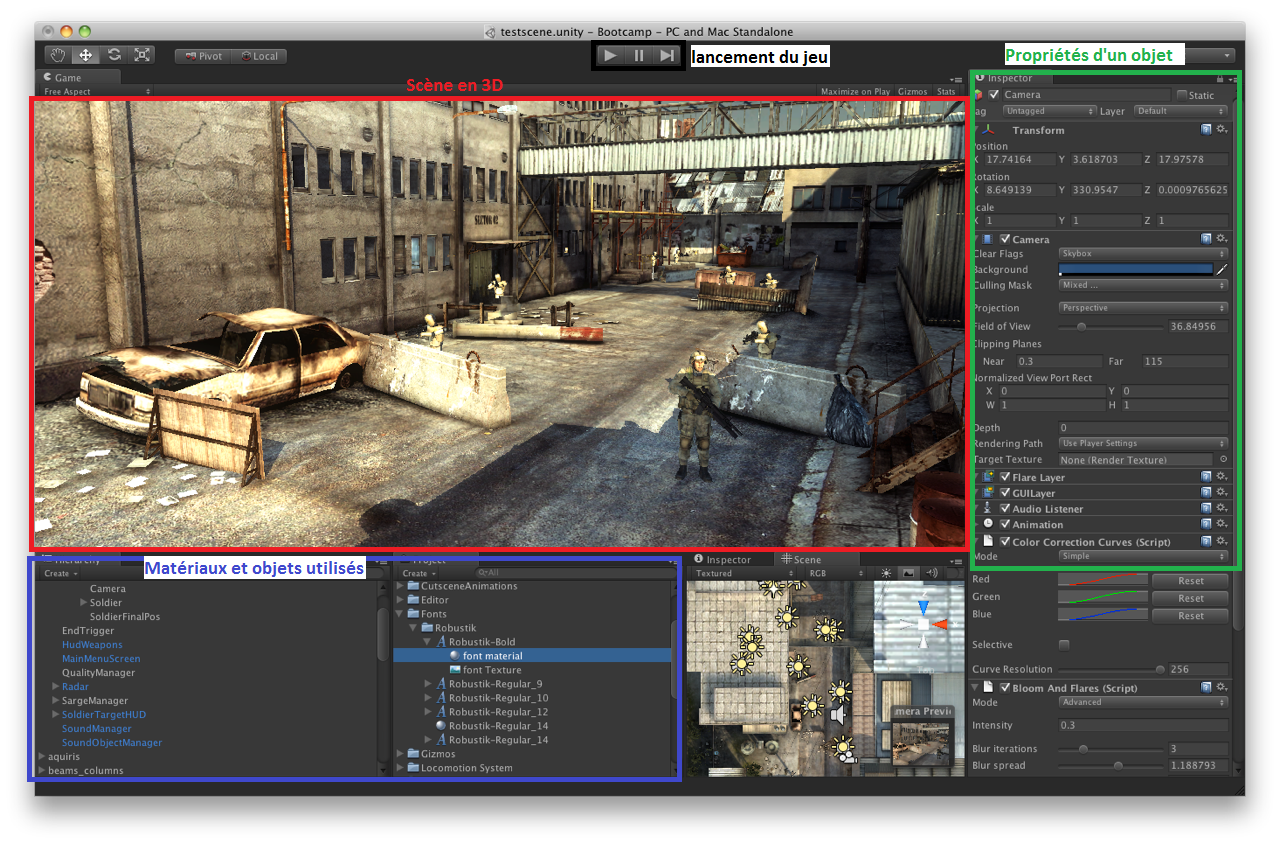
\includegraphics[scale=0.45]{./images/unity-3D_interface.png}
	\caption{Interface graphique de Unity3D}
	\end{figure}
	
	\newpage
	\subsection{Objets}
	\par Sur la scène nous venons de dire qu'il y a des \textit{GameObject}, et ils sont très importants. En effet, même un objet invisible dans le jeu peut être très utile.
	Les objets ou gameObjects on la particularité se voir greffer un certain nombre de composants, primitif à Unity3D ou non, qui eux même peuvent être modifiés. Voir \hyperlink{prefabTarget}{ici} pour aller encore plus loin avec les prefabs.

	\par Dans le projet nous avons des plans pour faire les murs et les écrans. Ils ont un matériau, qui lui possède une texture\footnote{Texture : Image sur laquelle les rayons lumineux vont se projeter}. Les plateformes, elles, sont brutes (sans matériaux) mais comme tous les objets visibles à l'écran elles possède un \textit{meshRenderer} qui leur permet de renvoyer les rayons lumineux. D'ailleurs c'est pour cette même raison que la caméra n'a pas de MeshRenderer. C'est aussi le cas pour l'objet \textit{Algorithm} qui lui ne possède qu'un script. Nous en parlerons dans une \hyperlink{prefabTarget}{section} dédiée.

	\subsection{Matériaux}
	\par Les matériaux sont une primitive de Unity3D et si nous avons décidé d'en parler c'est que dans la section qui suit, ils vont servir. Notamment à changer les cubes de couleur.\\
	C'est donc comme son nom l'indique, un composant\footnote{Composant : Nous appellerons dorénavant les primitives et script qu'on greffe à un GameObject : un composant, traduit de component dans Unity3D} indique comment la lumière va se refléter. Ils font intervenir des shaders que nous n'allons pas aborder dans se rapport.\\
	Un matériau à une couleur, un type de réfraction de la lumière (diffus ou/et spéculaire généralement) et une texture. La texture et la couleur son complémentaires. C'est-à-dire qu'on peut colorer une texture sans la modifier, juste par additivité avec la couleur du matériau.
	\begin{figure}[h]
	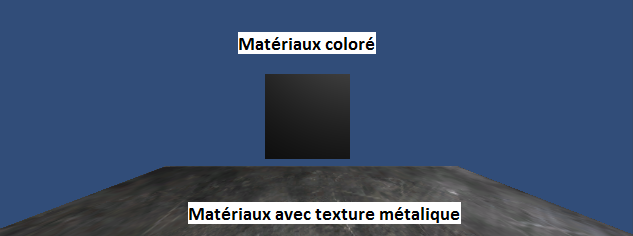
\includegraphics[scale=0.50]{./images/materiaux.png}
	\caption{Colorer avec ou sans texture}
	\end{figure}
	\par Exactement la même scène mais cette fois avec de la couleur dans le matériau en plus de la texture. On obtient un effet cuivré.
	\begin{figure}[h]
	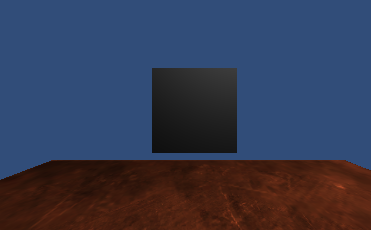
\includegraphics[scale=0.40]{./images/materiaux_cuivre.png}
	\caption{Modification de la composante MainColor du matériau}
	\end{figure}
	\par Dans cette exemple nous utilisons l'interface graphique pour obtenir ce résultat. Cela prend quelques minutes tout au plus. La bonne nouvelle est qu'il en va de même dans un script. Cela nécessite quelques minutes pour obtenir le même résultat. Et cela nous servira grandement pour colorier nos cubes.
	\newpage
	\section{Scripts}
	\hypertarget{scriptTarget}{Les} Scripts sont aussi des composants. Ils ont un rôle primordial dans la création du jeu, c'est d'ailleurs pour les créer que des développeurs sont nécessaires à la création de jeux vidéos.
	Dans cette section, nous aborderons le script qui est attaché à la caméra (rappel : un script est un composant et la caméra un gameObject). Il permet de saisir les objets, mais bien plus encore. Ensuite le script, cet fois beaucoup plus succinct, qui permet de maintenir et sauvegarder les objets dans leurs récepteurs. Enfin nous aborderons le script qui génère le rendu de l'algorithme.
	\subsection{Pour la caméra}
	Dans le projet il est nommé \textit{cameraGrabber} du fait qu'il permet de déplacer les objets. Initialement un autre script permettait de colorer le curseur lorsqu'on peut déplacer un objet, finalement il était plus judicieux de placer cette fonctionnalité   dans le script dont nous parlons. Nous n'allons pas détailler le listing du code, seulement les principales fonctions mais on le rappel : le code est disponible à l'adresse \href{https://github.com/manumanmax/SeriousVR.git}{https://github.com/manumanmax/SeriousVR.git} dans Assets/Scripts.
	
	\par D'abord le script utilise la méthode statique\footnote{Une méthode static peut être utilisée sans instanciation d'objet.} Physics.Raycast qui stock dans une variable de type RaycastHit le premier gameObject que le rayon percute. Mais avant on doit convertir le curseur dans les coordonnées du monde 3D. comme suit : 
	
	\lstset{style=sharpc}
\begin{lstlisting}
ray = Camera.main.ScreenPointToRay(new Vector3(cursorPos.x, cursorPos.y, 0.0f));
\end{lstlisting}
	Ainsi un prépare le rayon qu'on va lancer depuis le centre de l'écran. Qui est aussi la position du curseur. Une fois l'objet touché récupéré, on regarde si il à l'étiquette \textit{grabbable}, paramétrable dans les propriétés d'un objet.
	Si c'est le cas on rempli une texture en vert et on l'applique au centre de l'écran. Sinon on fait la même chose mais en rouge.
	
	\par Ensuite, on doit gérer le fait que les récepteurs d'objet on un effet scratch sur les cubes qu'on déplace. Pour expliquer cette partie, nous nous appuierons sur un vue de côté de la scène. Le jeu lancé et la fonction \textit{Debug.drawLine} affichant les traits de couleurs. Ils ne sont donc pas ajoutés sur l'image, ils sont produits en temps réel par l'application. Le vert est le vecteur qui représente la projection du curseur sur le plan de coordonnée z égal à l'objet qu'on déplace. Le rouge est la distance entre l'objet qui est donc verrouillé sur le récepteur et le curseur projeté.
	
	\begin{figure}[h]
	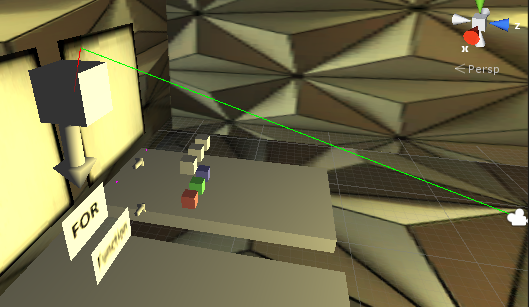
\includegraphics[scale=0.90]{./images/projection.png}
	\caption{Tracés de debug unity dans le cadre d'une projection selon une normale.}
	\end{figure}
	Nous en profiterons pour dire que les outils fournis par Unity3D pour débugger sont très utiles et assez bien pensés. \\Le code qui affiche les lignes est :
\lstset{style=sharpc}
	\begin{lstlisting}
	Debug.DrawLine(projection, transform.position, Color.green);
	Debug.DrawLine(projection, go.transform.position, Color.red);
	\end{lstlisting}
	\par Enfin avec ce vecteur représenté par le trait rouge. On peut savoir grâce à la méthode statique de Vector3, Distance, quel est la distance entre l'objet qu'on bouge et le récepteur. Le récepteur possède un halo dans lequel il attire l'objet, si on en sort on remet l'objet au niveau du curseur.
	\subsection{Pour stocker les objets des récepteurs}
	
	\par Plus simple, le script \textit{ReceiverScript} stock le cube qu'on à déposé dessus. Cela montre un autre aspect du scripting sous Unity3D. On peut stocker des variables ou des gameObjects pour que d'autres scripts y accès. C'est le cas pour le composant  \textit{ lockedObject } contenu dans ce script. La variable qui pointe sur l'objet est donc public, ce qui permettra au script de l'algorithme d'y accéder.
	\subsection{Pour l'algorithme}
	\par Pour rebondir sur le fait d'avoir prévu l'accès à l'objet des récepteurs nous allons introduire l'algorithme en lui même. Il est stocké dans un objet vide de la scène, sans quoi il ne serait jamais exécuté.\\
	Il nous vaut donc les objets stockés dans les récepteurs. On utilise une méthode dédié, inclue dans Unity3D comme ceci :
	\lstset{style=sharpc}
	\begin{lstlisting}
receivers = GameObject.FindGameObjectsWithTag("receiver");
	\end{lstlisting}
	\par On comprend donc qu'il faut, comme les cubes, paramétrer l'étiquette des récepteurs pour qu'ils soit reconnus par l'appel de cette méthode.\\
	Nous avons programmé les récepteurs pour qu'ils ne puissent recevoir qu'un certain type d'objet (incrément, valeur initiale, fonction etc). Donc on peut facilement vérifier que les récepteurs soit bien remplis afin d'être sûr que si on lance l'algorithme, il fonctionnera; même si les valeurs sont mauvaises.
	
	La boucle est générée en parsant\footnote{Parser : Le fait de regarder le contenu (ici) d'une chaine de caractère pour en tirer les informations qui nous intéressent.} le nom des objets sur les récepteurs. Une étape nécessaire au remplissage des paramètre de la fonction \textit{apply} du script. Cette méthode additionne les couleurs de la fonction avec la couleur d'initialisation comme suit : 
	\lstset{style=sharpc}
	\begin{lstlisting}
for (int i = 0; i < numberOfTimes; i += increment){
	cubes[i].renderer.material.color = (materials[i].color + initColor) / 2;
}
	\end{lstlisting}
	\par Ici on modifie l'attribut la couleur du matériau donc on peut aussi avoir des textures sur les cubes finales sans que ça n'impacte le jeu. 
	
	\section{Prefabs}
	\par \hypertarget{prefabTarget}{Les} Prefabs pour préfabriqué sont des objets ou groupements d'objets que l'on soit voir attribuer les même propriétés. Ils sont donc stockés directement dans un fichier. On peut ensuite les ajouter via l'interface ou par script. Il est intéressant de faire un objet type et une fois qu'il a des propriétés qui nous conviennent, on en fait un préfab pour le réutiliser dans autre scène.
	
	\subsection{Boucle}
	\par Pour réaliser la boucle, on a une imbrication de préfabs. La structure est un préfab, la boucle for est un préfab, les récepteurs sont des préfabs. Ainsi on peut dupliquer tout l'algorithme ou simplement un récepteur à partir du fichier correspondant. L'avantage est que lors qu'on change une propriété du préfab, les objets qui n'ont pas modifié cette propriété antérieurement sont tous affectés.
	\subsection{cubes}
	\par Les cubes sont un bon exemple de préfab. Ils possède un script, un tag, un matériau. On a donc tendance à copier coller ce genre d'objet fréquemment. Cependant lorsqu'on groupe les objets, si on change le nom du groupe, on ne veut pas que les sous éléments prennent tous le nom du groupe. C'est ce qui se passe pour toutes les propriété du préfab. Lorsqu'on ajoute un composant il est ajouté sur tous. Si on le modifie le préfab, seul les objets qui n'ont pas modifié ce composant sont modifiés.
	\begin{figure}[h]
	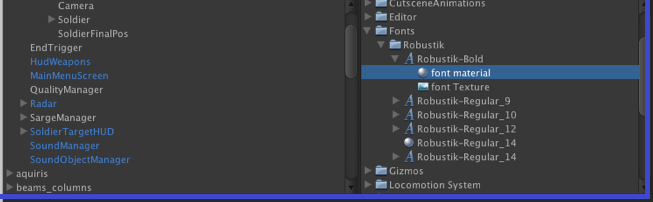
\includegraphics[scale=0.90]{./images/unity-3D_interface_zoom.png}
	\caption{Zoom Interface graphique de Unity3D}
	\end{figure}
	\par Dans ce zoom sur l'interface vu plus haut provenant d'un projet pris au hasard sur internet. On voit à gauche que les objets : HudWeapon, MainMenuScreen, Radar, SoldierTargetHUD, SoundManager et SoundObjectManager sont des préfabs. Les flèches avant le nom montre que ces préfabs contiennent plusieurs objets.
	
\chapter{Ajouts futures}
\section{De nouveaux niveau}
\par Avec les différentes fonctionnalités que propose le projet, il est déjà possible d'imaginer de nouveaux niveau. Plus difficiles et plus complets que le niveau 1.
\section{De nouveaux composants}
\par On peut imaginer de nouveaux composants qu'il faudrait ajouter au parseur. De nouvelles boucles comme la boucle \textit{tant que} peuvent être ajouter avec un script.\\
Cela nous conduit aussi à dire qu'on pourrait créer une notion d'héritage\footnote{Héritage : Processus dans le classe une classe reçois les attributs et les méthodes du classe qu'elle spécialise}. Cela permettrait de simplifier la création de nouveaux algorithme et boucles par spécialisation.
\section{Design}
\par Il est certains que le design de l'application et des composants peut être grandement amélioré. On peut imaginer des effets scriptés qui donnerait un aspect moins rustique au jeu.
\chapter{Difficultés}
\section{Prise en main}
\par La prise en main de Unity3D parait assez facile après coup. Mais cela n'a pas toujours été simple de travailler sans connaître toutes les possibilités qu'offrent Unity. Il ne faut surtout pas chercher à réinventer la roue car elle fait certainement déjà partie de l'API.
\section{Le dépôt git}
\par Nous n'avions jamais travailler avec git pour un projet Unity3D. Déjà pas parfaitement à l'aise avec git, il a fallut qu'un problème d'importation nous empêche d'utiliser l'interface de Unity. Sans quoi les dossier que l'on récupérait depuis GitHub ne fonctionnaient pas.\\
Au final, il faut inclure tous les fichier sans se poser de question sur le dépôt et cela fonctionne parfaitement.
\section{Difficultés techniques}
\par Lorsque l'on déplace un corps rigide (RigidBody), une imprécision peut faire que la position visualisée à l'écran n'est pas la position de l'objet. C'est probablement un bog corrigé dans la dernière version de Unity3D (version 5). Visuellement quand on déplaçait un objet, parfois, il tombait. Donc lorsqu'on le lâchait, il disparaissait du champ de la caméra.\\
\par Le curseur à posé énormément de problème. Toutes les méthodes disponible sur internet utilise la position du curseur comme référence. Honnêtement il est peut probable qu'un FPS utilise cette position car elle est relative à la position de la souris. Cela nécessite de verrouiller le curseur etc. Donc une solution simple est de supprimer la souris et de placer une texture au centre de l'écran. Cette texture représente notre curseur et la caméra pointe toujours dans sa direction. Cette méthode à corrigé tous les problèmes liées à aux position des objets parfois houleuses.
\chapter{Apports personnels}
\par Emmanuel : Même si le temps à manqué, j'ai acquis bon nombre de compétences dans ce projet. D'abord, la connaissance de deux nouvelles technologies : Unity3D et l'OculusVR. J'ai aussi à ma grande surprise, découvert Visual Studio, du fait qu'on avait pas d'autre choix que de développer sous Windows et que MonoDevelop ne me plaisait pas.\\
Ensuite cela m'a permis une fois de plus de voir qu'il faut beaucoup de temps pour intégrer les mécanisme d'une grande API comme celle proposée par Unity. Et cela me plaît beaucoup aujourd'hui d'en savoir plus. Car je suis certains que je m'en servirais régulièrement à l'avenir.\\
J'ai pu aborder rapidement le C\#, qui m'a bien plu. Même si je n'ai pas pu utiliser l'aspect objet du langage dans le projet.\\
Je dirais enfin qu'un projet réalisé à 2 sur un an est difficile à mettre en place. Même si on identifie les risque, le plus risque c'est de ne pas réussi à développer les fonctionnalité nécessaires à un sprint dans le temps imparti. Cela affect tout le projet et sa conduite.

\listoffigures
\end {document}
